% \documentclass{beamer}
\documentclass[xcolor=dvipsnames]{beamer}
\usefonttheme{serif}
%% \usecolortheme[named=Blue]{structure}
\setbeamersize{text margin left=30mm, text margin right=30mm}
\useoutertheme{infolines}
%% \usetheme[height=7mm]{Rochester}
\usetheme{Pittsburgh}
\setbeamertemplate{items}[ball]
\setbeamertemplate{blocks}[rounded][shadow=true]
\setbeamertemplate{navigation symbols}{}

\usepackage[utf8x]{inputenc}
%% \usepackage{default}
\usepackage[english]{babel}
\usepackage{geometry}
%% \usepackage{fullpage}
\usepackage{amsmath, amsthm, amssymb}
\usepackage{listings}
\usepackage{pxfonts}
%% \usepackage{caption}
\usepackage[labelformat=empty]{caption}
\usepackage{amsmath}

%% \usepackage{xcolor}
%% \usepackage{newunicodechar}
%% \newcommand\Warning{%
%%  \makebox[1.4em][c]{%
%%  \makebox[0pt][c]{\raisebox{.1em}{\small!}}%
%%  \makebox[0pt][c]{\color{red}\Large$\bigtriangleup$}}}%
%% \newunicodechar{⚠}{\Warning}


%% \usepackage{color}
%% \usepackage{graphicx}
%% \usepackage{natbib}
%% \usepackage{array}
%% \usepackage{booktabs}
%% \usepackage{tabu}
%% \usepackage[utf8]{inputenc}
%% \usepackage{fancyhdr}
%% \usepackage{float}
%% \usepackage{subfigure}
%% \usepackage{titlesec}

\setbeamertemplate{headline}{}
\setbeamertemplate{footline}[frame number]{}
\setbeamertemplate{navigation symbols}{}
\setbeamertemplate{footline}{}
\setbeamertemplate{footline}[frame number]


\def\CCT{{C\nolinebreak[4]\hspace{-.05em}\raisebox{.4ex}{\tiny\bf ++}}}
\def\CC{{C\nolinebreak[4]\hspace{-.05em}\raisebox{.4ex}{\small\bf ++}}}


\definecolor{lstgray}{gray}{0.93}
\definecolor{strgray}{gray}{0.4}

\lstset{ %
  escapechar=@,
  language=C++,
  basicstyle=\footnotesize\ttfamily,
  %% basicstyle=\ttfamily,
  stringstyle=\color{strgray}\ttfamily,
  commentstyle=\color{OliveGreen}\ttfamily,
  %% morecomment=[l][\color{red}]{\#},
  morecomment=[l][\color{blue}]{\#},
  backgroundcolor=\color{lstgray},
  frame=f,
  frameround=ffff,
  tabsize=2,
  breaklines=true,
  breakatwhitespace=false,
  showspaces=false,
  showstringspaces=false,
  xleftmargin=5pt,
  xrightmargin=5pt,
  morekeywords={decltype,sizeof,constexpr},
  %% keywordstyle=\color{red},
  keywordstyle=\bfseries\color{black}\ttfamily,
  keywords=[2]{Option,PRIMAL,TANGENT,ADJOINT},
  keywordstyle=[2]\bfseries\color{OliveGreen}\ttfamily,
  keywords=[3]{Drv,mode,SDrv,EDrv,DrvFieldLoop\_begin,DrvFieldLoop\_end,drv,find\_DrvMode,DrvMode,edrv,primal,DrvVariadicNode,ScopedExprBinding},
  keywordstyle=[3]\color{blue}\ttfamily,
  keywords=[4]{Discrimiant,discrimiant,Hyp,hyp,MeanSd,mean\_sd,evaluate},
  keywordstyle=[4]\color{red}\ttfamily,
}

\def\redcolor{\color{red}}
\def\bluecolor{\color{blue}}
\def\blackcolor{\color{black}}
\def\graycolor{\color{gray}}
\def\greencolor{\color{OliveGreen}}


\def\sectionname{\translate{Section}}
\def\insertsectionnumber{\arabic{section}}
\setbeamertemplate{section page}
{
  \begin{centering}
    \begin{beamercolorbox}[sep=4pt,center]{part title}
      \usebeamerfont{section title}\insertsection\par
    \end{beamercolorbox}
  \end{centering}
}
\def\sectionpage{\usebeamertemplate*{section page}}


\AtBeginSection{\frame{\sectionpage}}


\title{Recursive compile time adjoint in \CC}
\subtitle{23\textsuperscript{rd} EuroAD Workshop}
\author{Dominic Jones}
\date{\small{11--13 Aug 2020}}
\institute{\small{Siemens PLM, London}\\\small{\texttt{dominic.jones@cd-adapco.com}}}

\begin{document}
\begin{frame}[plain]
  \titlepage
\end{frame}


\begin{frame}[fragile]{Introduction}
\begin{itemize}
\item[--] The compile time differentiation of a {\CC} function which only calls built-in functions has been demonstrated in previous talks. \vspace{3mm}
\item[--] This talk describes the approach for differentiating a function which may call any nested function. \vspace{3mm}
\item[--] Siemen's Simcenter Star-CCM+ simulation software has an implementation of this approach, and is used to differentiate the Spalart Allmaras turbulence model, among other things. \vspace{3mm}
\end{itemize}
\end{frame}




\begin{frame}[fragile]{What's new}
  \begin{columns}[T] % align columns
    \begin{column}{0.44\textwidth}
      {\color{gray}{\; Flat structure (old)}}
      \begin{lstlisting}
hypotenuse(A const &a,
           B const &b,
           R &r)
{
  auto a2 = a * a;
  auto b2 = b * b;
  auto d = a2 + b2;
  r = sqrt(d);
}
  \end{lstlisting}
    \end{column}%
    \hfill%
    \begin{column}{0.56\textwidth}
      {\color{gray}{\; Nested structure (new)}}
        \begin{lstlisting}
hypotenuse(A const &a,
           B const &b,
           R &r)
{
  auto d = discrimiant(a, b);
  r = sqrt(d);
}
  \end{lstlisting}
  
  \begin{lstlisting}
discrimiant(A const &a,
            B const &b)
{
  auto a2 = a * a;
  auto b2 = b * b;
  return a2 + b2;
}
  \end{lstlisting}
    \end{column}%
  \end{columns}
\end{frame}


\section{Built-in functions}


\begin{frame}[fragile]{Hypotenuse}
\begin{equation*}
  r = \sqrt{a^2 + b^2}
\end{equation*}

\begin{lstlisting}
float a = 3;
float b = 4;
float r;

{
  auto d = a*a + b*b;
  r = sqrt(d);
}

std::cout << r << std::endl;  // r = 5
\end{lstlisting}
\end{frame}


\begin{frame}[fragile]{Primal of Hypotenuse}
\begin{equation*}
  r = \sqrt{a^2 + b^2}
\end{equation*}

\begin{lstlisting}
float a = 3;
float b = 4;
float r;

auto constexpr mode = DrvMode::PRIMAL;

Drv<mode, float>  a_{a};  // input
Drv<mode, float>  b_{b};  // input
Drv<mode, float&> r_{r};  // output

{
  auto d = a_*a_ + b_*b_;
  r_ = sqrt(d);
}

std::cout << r << std::endl;  // r = 5
\end{lstlisting}
\end{frame}


\begin{frame}[fragile]{Tangents of Hypotenuse}
\begin{equation*}
  \frac{d r}{d a}
\end{equation*}

\begin{lstlisting}
float a = 3, a_drv = 1;  // w.r.t. `a'
float b = 4, b_drv = 0;
float        r_drv;

auto constexpr mode = DrvMode::TANGENT;

Drv<mode, float>  a_{a, a_drv};
Drv<mode, float>  b_{b, b_drv};
Drv<mode, float&> r_{r_drv};

{
  auto d = a_*a_ + b_*b_;
  r_ = sqrt(d);
}

std::cout << r_drv << std::endl;  // dr/da = 0.6
\end{lstlisting}
\end{frame}


\begin{frame}[fragile]{Tangents of Hypotenuse}
\begin{equation*}
  \frac{d r}{d b}
\end{equation*}

\begin{lstlisting}
float a = 3, a_drv = 0;
float b = 4, b_drv = 1;  // w.r.t. `b'
float        r_drv;

auto constexpr mode = DrvMode::TANGENT;

Drv<mode, float>  a_{a, a_drv};
Drv<mode, float>  b_{b, b_drv};
Drv<mode, float&> r_{r_drv};

{
  auto d = a_*a_ + b_*b_;
  r_ = sqrt(d);
}

std::cout << r_drv << std::endl;  // dr/db = 0.8
\end{lstlisting}
\end{frame}


\begin{frame}[fragile]{Adjoint of Hypotenuse}
\begin{equation*}
\begin{bmatrix}
\frac{d r}{d a} & \frac{d r}{d b}
\end{bmatrix}^T
\end{equation*}

\begin{lstlisting}
float a = 3, a_drv = 0;
float b = 4, b_drv = 0;
float        r_drv = 1;  // w.r.t. `r'

auto constexpr mode = DrvMode::ADJOINT;

Drv<mode, float>  a_{a, a_drv};
Drv<mode, float>  b_{b, b_drv};
Drv<mode, float&> r_{r_drv};

{
  auto d = a_*a_ + b_*b_;
  r_ = sqrt(d);
}

std::cout << a_drv << std::endl;  // dr/da = 0.6
std::cout << b_drv << std::endl;  // dr/db = 0.8
\end{lstlisting}
\end{frame}


\section{User defined functions}


\begin{frame}[fragile]{Defining a function}
\begin{lstlisting}
struct Discrimiant
{
  template<DrvMode mode>  // `float' could be templated, too
  static void
  evaluate(Drv<mode, float> const &a,
           Drv<mode, float> const &b,
           Drv<mode, float&> r)
  {
    auto a2 = a * a;
    auto b2 = b * b;
    r = a2 + b2;
  }
};
\end{lstlisting}
\begin{itemize}
\item[--] All function arguments are treated as differentiable terms, even if in the function body some may be treated passively, e.g.
\begin{lstlisting}
auto a2 = primal(a * a);  // i.e.  float a2 = a * a;
\end{lstlisting}
\end{itemize}
\end{frame}


\begin{frame}[fragile]{Calling it via a free function}
\begin{lstlisting}
template<typename E0, typename E1>
auto
discrimiant(E0 &&e0, E1 &&e1)
->
DrvVariadicNode<GetDrvMode<E0, E1>::value,   // mode
                decltype(primal(e0 + e1)),   // result
                Bind_evaluate<Discrimiant>,  // operator
                E0, E1>                      // children
{
  return {std::forward<E0>(e0), std::forward<E1>(e1)};
}
\end{lstlisting}
\end{frame}


\begin{frame}[fragile]{Unified call syntax}
\begin{lstlisting}
Drv<mode, float>  a_{a, a_drv};
Drv<mode, float>  b_{b, b_drv};
Drv<mode, float&> r_{r_drv};

{
  auto d = discrimiant(a_, b_);
  r_ = sqrt(d);
}
\end{lstlisting}

\begin{itemize}
\item[--] {\color{red}\texttt{discrimiant}} can be used just like any built-in function,\newline such as \texttt{sqrt}. \vspace{3mm}
\item[--] \texttt{a\_} or \texttt{b\_} could be replaced with \texttt{a} or \texttt{b}, respectively, to treat either passively. \vspace{3mm}
\end{itemize}
\end{frame}


\section{The variadic expression node}


\begin{frame}[fragile]{Unary, binary, \ldots and \emph{variadic}}
\begin{itemize}
\item[--] Allied with variadic templates, perfect forwarding and \texttt{std::tuple}, unary and binary expression nodes can be generalised into an \emph{N-}ary form. \vspace{3mm}
\item[--] In principle, all built-in functions, such as \texttt{+ - * /} \; and \; \texttt{sin cos tan pow}, could return an \emph{N-}ary node. \vspace{3mm}
\item[--] A mechanism to distinguish between built-in and user defined functions is still required. This is done with an operator binding, such as \texttt{Bind\_evaluate<OP>}.
\end{itemize}
\end{frame}


\begin{frame}[fragile]{Base of all nodes}
\begin{lstlisting}
template<DrvMode m, typename R, typename E>
struct DrvExpression
{
  static constexpr auto mode = m;
  using Result = R;
  using Expression = E;
};
\end{lstlisting}
\end{frame}


\begin{frame}[fragile]{Variadic node*}
\begin{lstlisting}
template<DrvMode m,          // mode
         typename R,         // result
         typename OP,        // operator
         typename... EE>     // children
struct DrvVariadicNode
  : DrvExpression<m, R, DrvVariadicNode>
{
  DrvVariadicNode(EE &&... ee) : _ee(ee...) {}

  template<int I> auto const &node() const {
    return std::get<I>(_ee);
  }

  private: std::tuple<EE...> _ee;
};
\end{lstlisting}
\end{frame}


\begin{frame}[fragile]{Variadic node}
\begin{itemize}
\item[--] The \emph{N-}ary node is minimal, providing nothing more than access to its children.  \vspace{3mm}
\item[--] Children will be associated to the node by value, for in-place expressions or literals, or by reference. This difference is distinguished by perfect forwarding. \vspace{3mm}
\item[--] The values and references are held in the \texttt{std::tuple} member. \vspace{3mm}
\end{itemize}
\end{frame}


\begin{frame}[fragile]{Evaluating the primal*}
\begin{lstlisting}
template<DrvMode m,
         typename OP, typename R, typename... EE,
         typename AA, int... I>
auto
evaluatePrimal(
  DrvVariadicNode<m, R, OP, EE...> const &expr,
  AA const &aa,                        // primal values: a, b
  std::index_sequence<I...>)
{
  auto constexpr lm = DrvMode::PRIMAL; // local mode
  auto r_pri = R(0);
  
  OP::evaluate(
    Drv<lm, decltype(DrvVariadicNode::node<I>())::Result>
      {std::get<I>(aa)}...,            // inputs
    Drv<lm, R&>{r_pri});               // output
    
  return r_pri;
}
\end{lstlisting}
\end{frame}


\begin{frame}[fragile]{Evaluating the primal}
\begin{itemize}
\item[--] All work relating to differentiable expressions is done by free functions.\vspace{3mm}
\item[--] The expression mode, \texttt{m}, is distinguished from the local mode, \texttt{lm}, in order to generate the correct instance of the user defined function. \vspace{3mm}
\item[--] The arguments for \texttt{OP::evaluate} are constructed in-place, generating a new (and independent) differentiation context inside the user defined function.  \vspace{3mm}
\end{itemize}
\end{frame}


\begin{frame}[fragile]{Evaluating the adjoint*}
\begin{lstlisting}
template<DrvMode m,
         typename OP, typename R, typename... EE,
         typename AA, typename RHS, int... I>
void
evaluateAdjoint(
  DrvVariadicNode<m, R, OP, EE...> const &expr,
  AA const &aa,               // primal values: a, b
  AA &aa_drv,                 // adjoint refs:  a_drv, b_drv
  RHS const &rhs,             // seed value:    r_drv
  std::index_sequence<I...>)
{
  OP::evaluate(
    Drv<m, decltype(DrvVariadicNode::node<I>())::Result>
      {std::get<I>(aa), std::get<I>(aa_drv)}...,
    Drv<m, R&>{rhs});
}
\end{lstlisting}
\end{frame}


\begin{frame}[fragile]{Evaluating the adjoint}
\begin{itemize}
\item[--] Here, \texttt{OP::evaluate} is compiled in adjoint mode, as deduced from the arguments.  \vspace{3mm}
\item[--] Despite the fact that \texttt{OP::evaluate} will have been evaluated in primal mode already, the values of any intermediate results cannot be captured and used here because there is no monolithic expression tree `view'. \vspace{3mm}
\item[--] The work presented in EuroAD 2019 did have such a view, and so avoided duplicate primal evaluations. But compilation time proved to be too expensive. \vspace{3mm}
\end{itemize}
\end{frame}


\begin{frame}[fragile]{Summary}
\begin{itemize}
\item[--] The variadic template expression node, combined with perfect forwarding, facilitates generic user defined functions. \vspace{3mm}
\item[--] User defined virtual functions can be supported, and so too functions with multiple results. \vspace{3mm}
\item[--] Despite being difficult to implement, the added functionality of variadic nodes has proved to be a major advancement in deploying automatic differentiation in Star-CCM+.  \vspace{3mm}
\item[--] The tool is fully \texttt{constexpr} qualified, and with aggressive compiler optimisations performs very well: 2.82x on the harmonic test (331 nodes, 5 inputs); cf. EuroAD 2019. \vspace{3mm}
\end{itemize}
\end{frame}


%%
\begin{frame}[plain]
  \titlepage
\end{frame}


\end{document}







\section{\texttt{l-value} types}


\begin{frame}[fragile]{Named approach}
\begin{lstlisting}
{
  EDrv<mode, float> d = a*a + b*b;
  r = sqrt(d);
}
\end{lstlisting}

\begin{itemize}
\item[--] \texttt{EDrv<>} doesn't know the type of the expression: \texttt{a*a + b*b} \vspace{3mm}
\item[--] In order for \texttt{EDrv<>} to make a copy of the expression so as to evaluate its adjoint during destruction, \texttt{OpaqueObjectManager} is used \vspace{3mm}
\item[--] The manager provides a stack buffer. If the expression is larger than the buffer then the heap is used \vspace{3mm}
\end{itemize}
\end{frame}


\begin{frame}[fragile]{\texttt{auto} approach}
\begin{lstlisting}
{
  auto d = edrv(a*a + b*b);
  r = sqrt(d);
}
\end{lstlisting}

\begin{itemize}
\item[--] \texttt{auto} knows the type of the expression: \texttt{a*a + b*b} \vspace{3mm}
\item[--] \texttt{auto} holds a copy of the expression so as to evaluate its adjoint during destruction \vspace{3mm}
\item[--] \texttt{auto} and \texttt{edrv} go together, rather like \texttt{std::unique\_ptr} and \texttt{std::make\_unique} \vspace{3mm}
\item[--] This approach produces the most efficient code
\end{itemize}
\end{frame}


\begin{figure}[H]
 \centering
 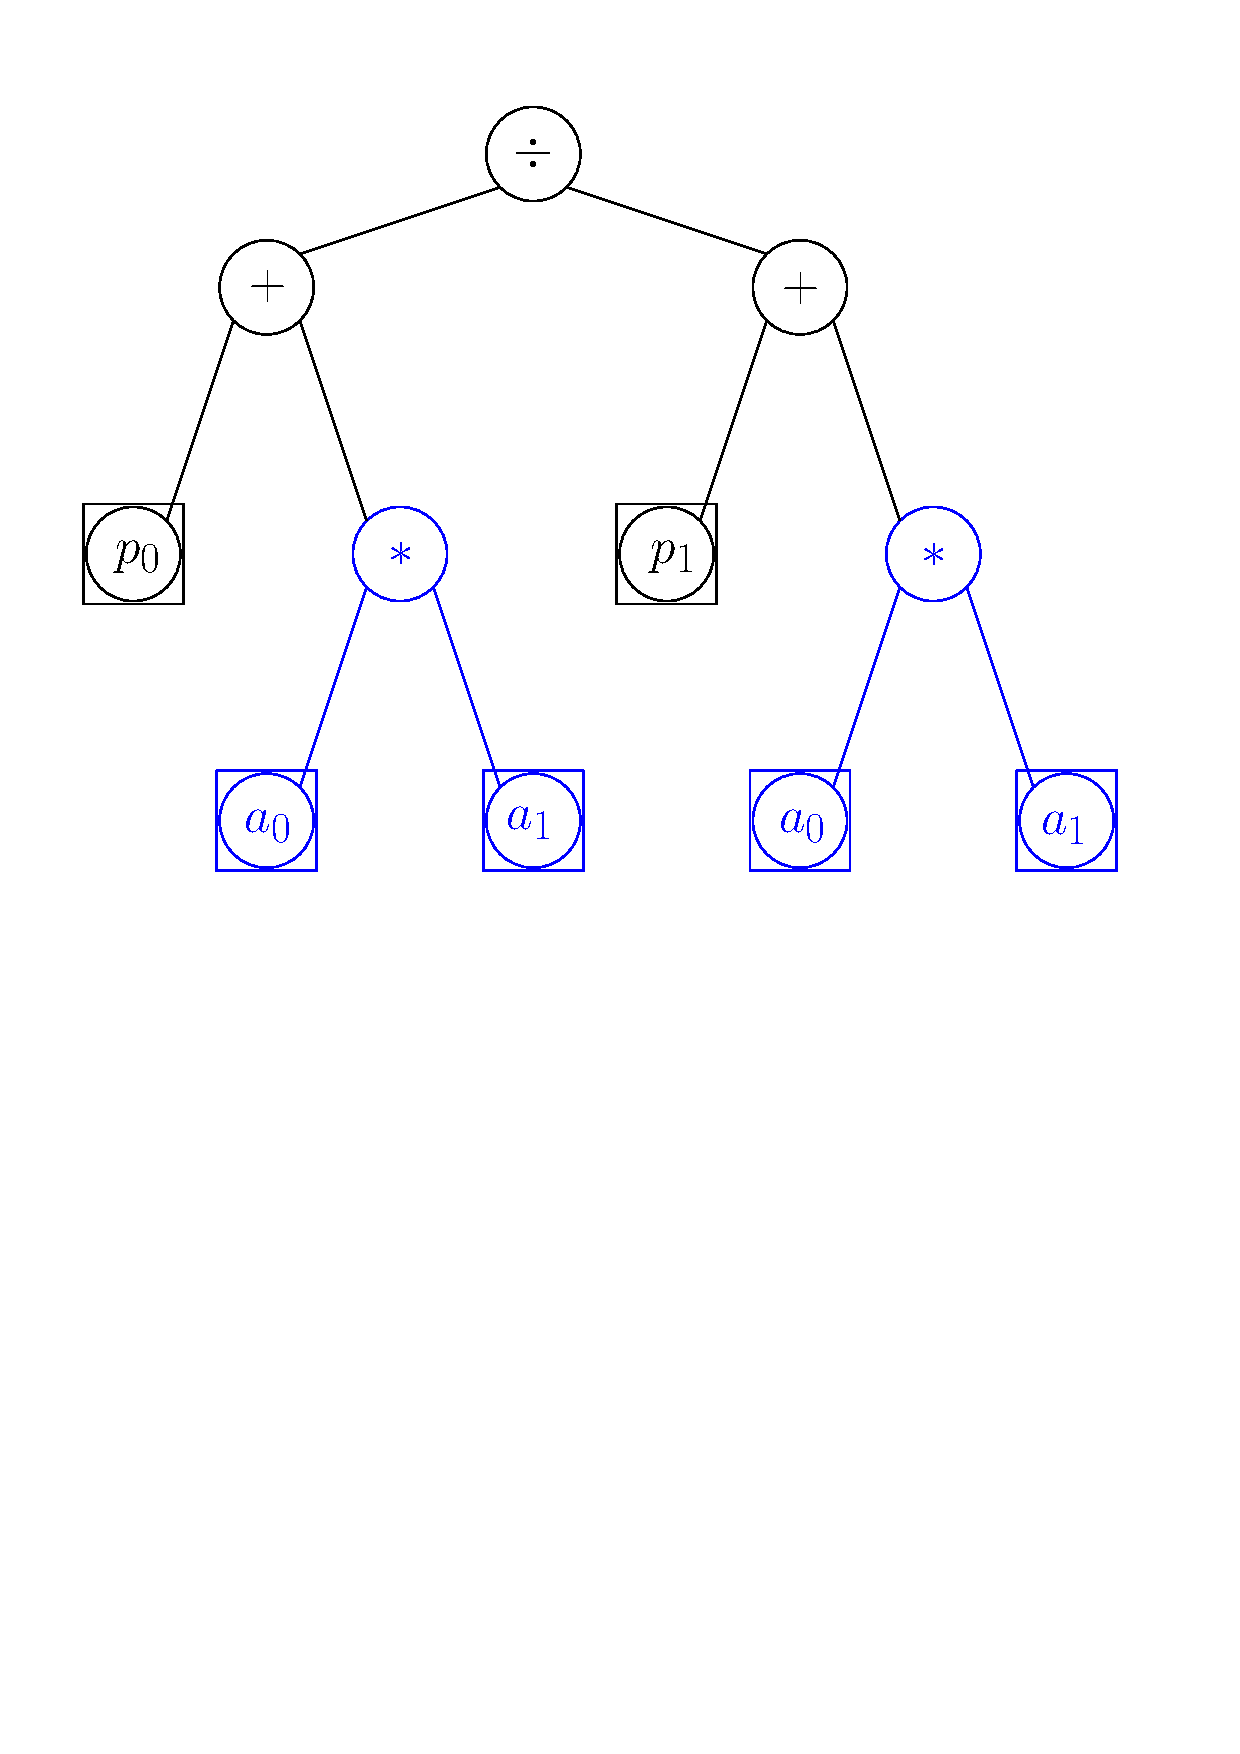
\includegraphics[width=0.99\textwidth]{fig_exprtree_dup}
\end{figure}



Abstract

Various attempts have been made at CD-adapco/Siemens to develop a suitable AD tool for the fluid dynamics simulation software Star-CCM+. This work presents the latest iteration and is considered a synthesis of several years work.

The approach developed leverages a number of language features found in C++14 in order to differentiate a top-level function, which in tern will cause the differentiation of arbitrary nested functions.

Nested functions are facilitated by having them construct an expression node from a generic node template taking an arbitrary number of parameters. The approach enables them to be treated in a similar way to built-in functions.

The generic approach to handling nested functions has proved invaluable to the development of the adjoint models in Star-CCM+, particularly with the added capacity to support arbitrary virtual functions.





\section{The essential language feature}


\begin{frame}[fragile]{Perfect forwarding}
\begin{lstlisting}
template<class OP, class E0>
struct Unary { Unary(E0 &&e0) {} };
\end{lstlisting}

\begin{lstlisting}
class Sqrt;

template<class E0>
auto sqrt(E0 &&e0)
{
  return Unary<Sqrt, E0>(std::forward<E0>(e0));
}
\end{lstlisting}

\begin{lstlisting}
float const a0{1};
auto a1 = sqrt(a0);        // Unary<Sqrt, float const &>

float b0{1};
auto b1 = sqrt(b0);        // Unary<Sqrt, float &>

auto c1 = sqrt(float{1});  // Unary<Sqrt, float>
\end{lstlisting}
\end{frame}


\section{What's new}



\begin{frame}[fragile]{Star-CCM+ adjoint}
\begin{figure}[H]
 \centering
 \includegraphics[width=0.99\textwidth]{starccm}
\end{figure}
\end{frame}


\begin{frame}[fragile]{Star-CCM+ compilation (ref)}
\begin{figure}[H]
 \centering
 \includegraphics[width=0.9\textwidth]{current.png}
\end{figure}
\end{frame}


\begin{frame}[fragile]{Star-CCM+ compilation (AD v1)}
\begin{figure}[H]
 \centering
 \includegraphics[width=0.9\textwidth]{unified_roe_auto_rev1.png}
\end{figure}
\end{frame}


\begin{frame}[fragile]{Star-CCM+ compilation (AD v2)}
\begin{figure}[H]
 \centering
 \includegraphics[width=0.9\textwidth]{unified.png}
\end{figure}
\end{frame}
